\documentclass[12pt]{article}
\usepackage[margin=2.5cm]{geometry}
\usepackage{enumerate}
\usepackage{amsfonts}
\usepackage{amsmath}
\usepackage{fancyhdr}
\usepackage{amsmath}
\usepackage{amssymb}
\usepackage{amsthm}
\usepackage{mdframed}
\usepackage{graphicx}
\usepackage{subcaption}
\usepackage{adjustbox}
\usepackage{listings}
\usepackage{xcolor}
\usepackage{courier}
\usepackage[utf]{kotex}
\usepackage{hyperref}
\usepackage{soul}

\definecolor{codegreen}{rgb}{0,0.6,0}
\definecolor{codegray}{rgb}{0.5,0.5,0.5}
\definecolor{codepurple}{rgb}{0.58,0,0.82}
\definecolor{backcolour}{rgb}{0.95,0.95,0.92}

\lstdefinestyle{mystyle}{
    backgroundcolor=\color{backcolour},
    commentstyle=\color{codegreen},
    keywordstyle=\color{magenta},
    numberstyle=\tiny\color{codegray},
    stringstyle=\color{codepurple},
    basicstyle=\ttfamily\footnotesize,
    breakatwhitespace=false,
    breaklines=true,
    captionpos=b,
    keepspaces=true,
    numbers=left,
    numbersep=5pt,
    showspaces=false,
    showstringspaces=false,
    showtabs=false,
    tabsize=1
}

\lstset{style=mystyle}

\pagestyle{fancy}
\renewcommand{\headrulewidth}{0.4pt}
\lhead{CSC 369}
\rhead{Midterm 3 Notes}

\begin{document}
\title{CSC 369 Midterm 3 Notes}



\section*{Index-based File System}

\begin{center}

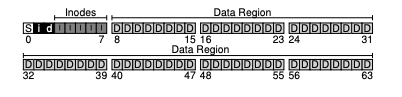
\includegraphics[width=\linewidth]{../images/midterm_2_solution_20.png}
\end{center}

\begin{itemize}
    \item Has following parts

    \begin{itemize}
        \item Superblock
        \item Inode Bitmap
        \item Data Bitmap
        \item Inodes
        \item Data Region
    \end{itemize}

    \item Each block in file system is 4KB
    \item Uses a large amount of metadata per file (especially for large files)
\end{itemize}

\section*{Superblock}

\begin{center}
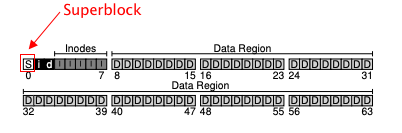
\includegraphics[width=\linewidth]{../images/midterm_2_solution_21.png}
\end{center}

\begin{itemize}
    \item contains information about the file system, including

    \begin{enumerate}[1.]
        \item the number of inodes and data blocks in a particular file system
        \item the magic number of some kind to identify the file system type (e.g NFS, FFS, VSFS)
    \end{enumerate}

    \item The OS reads superblock \underline{first} to initialize various parameters,
    and then attach volume to the file-system tree
\end{itemize}

\section*{Bitmap}

\begin{center}
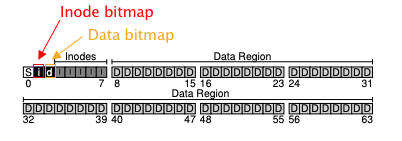
\includegraphics[width=\linewidth]{../images/midterm_2_solution_22.png}
\end{center}

\begin{itemize}
    \item Tracks whether inode or data blocks are free or allocated
    \item Is a simple and popuar structure
    \item Uses each bit
    \begin{itemize}
        \item \texttt{0} means free
        \item \texttt{1} means in use
    \end{itemize}

    \item \textbf{Data Bitmap} is bitmap for data region
    \item \textbf{Inode Bitmap} is bitmap for inode region
\end{itemize}

\section*{Inode}

\begin{center}
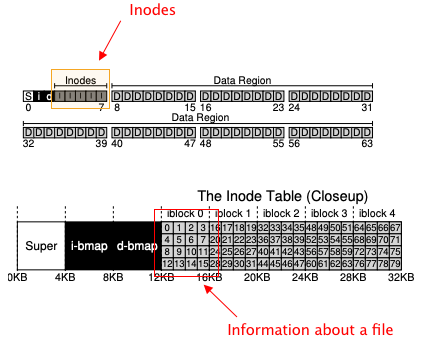
\includegraphics[width=\linewidth]{../images/midterm_2_solution_23.png}
\end{center}

\begin{itemize}
    \item Is a short form for \textbf{index node}
    \item Contains disk block location of the object's data $^{[7]}$
    \item Contains all the information you need about a file (i.e. metadata)

    \begin{itemize}
        \item File Type
        \begin{itemize}
            \item e.g. regular file, directory, etc
        \end{itemize}
        \item Size
        \item Number of blocks allocated to it
        \item Protection information
        \begin{itemize}
            \item such as who owns the file, as well as who can access it
        \end{itemize}
        \item Time information
        \begin{itemize}
            \item e.g. When file was created, modified, or last accessed
        \end{itemize}
        \item Location of data blocks reside on disk
    \end{itemize}
\end{itemize}

\section*{Data Region}

\begin{center}
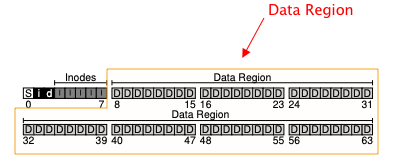
\includegraphics[width=\linewidth]{../images/midterm_2_solution_24.png}
\end{center}

\begin{itemize}
    \item Is the region of disk we use for user data
\end{itemize}


\section{Block}

\begin{itemize}
    \item Size of each block is 4KB
\end{itemize}

\section{lseek}

\begin{itemize}
    \item \textbf{Syntax:} \texttt{off\_t lseek(int fildes, off\_t offset, int whence)}

    \begin{itemize}
        \item \texttt{fildes} - file descriptor
        \item \texttt{offset} - file offset to a particular position in file
    \end{itemize}
\end{itemize}

\section{Kilobyte}

\begin{itemize}
    \item 1 kilobyte is \underline{1024 bytes}
\end{itemize}

\section{file}
\begin{itemize}
    \item is an array of bytes which can be created, read, written and deleted
    \item low-level name is called \textbf{inode number} or \textbf{i-number}
\end{itemize}
\section{Reading a File From Disk}

\bigskip

\underline{\textbf{Example}}

\bigskip

When

\bigskip

\texttt{open("/foo/bar", O\_READONLY)}

\bigskip

is called

\bigskip

\begin{itemize}
    \item the goal is to find the inode of the file \texttt{bar} to read its basic information
    (i.e. includes permission, information, file size etc)
    \item done by traversing the pathname and locate the desired inode
    \item Steps

    \begin{enumerate}[1.]
        \item Begin traversal at the root of the file system, in the \textbf{root directory}

        \item Find \textbf{inode} of the root directory by looking for \texttt{i-number}

        \begin{itemize}
            \item \textbf{i-number} is found in it's parent directoy
            \item for root directory, there is no parent directory
            \item it's inode number is 2 (for UNIX file systems)
        \end{itemize}

        \item Read the \textbf{inode} of root directory
        \item Once its \textbf{inode} is read, look inside to find pointers
        to data blocks
        \item Recursively traverse the pathname until the desired inode is found (e.g \texttt{foo} $\to$ \texttt{bar})
        \item Issue a \texttt{read()} system call to read from file

        \begin{itemize}
            \item \texttt{fd} with offset \texttt{0} reads the first file block (e.g. \texttt{bar data[0]})
            \item \texttt{lseek(..., offset\_amt * size\_of\_file\_block)} is used to offset/move to desired block in \texttt{bar}
        \end{itemize}

        \item Trasnfer data to \texttt{buf} data block

        \item Close \texttt{fd}. No I/O is read.
    \end{enumerate}
\end{itemize}

\section{inode}

\begin{itemize}
    \item total size may vary
    \item inode pointer has size of 4 byte
    \item Has 12 \textbf{direct pointers} to 4KB data blocks
    \item Has 1 \textbf{indirect pointer} [when file grows large enough]
    \item Has 1 \textbf{double indirect Pointer} [when file grows large enough]
    \item Has 1 \textbf{triple indirect Pointer} [when file grows large enough]
\end{itemize}

\section{Indirect Pointers}

\begin{itemize}
    \item Is allocated to data-block if file grows large enough
    \item Has total size of 4 KB or 4096 bytes
    \item Has $4096/4 = 1024$ pointers
    \item Each pointer points to 4KB data-block
    \item File can grow to be $(12 + 1024) \times 4\text{K} = 4144\text{KB}$
\end{itemize}

\section{Double Indirect Pointers}

\begin{itemize}
    \item is allocated when single indirect pointer is not large enough
    \item each pointer in first pointer block points to another pointer block
    \item has $1024^2$ pointers
    \item each of $1024^2$ pointers point to 4KB data block
    \item File can grow to be $(12 + 1024 + 1024^2) \times 4\text{K} = 4198448\text{KB}$ or $\approx 4.20 \text{GB}$

    \begin{center}
    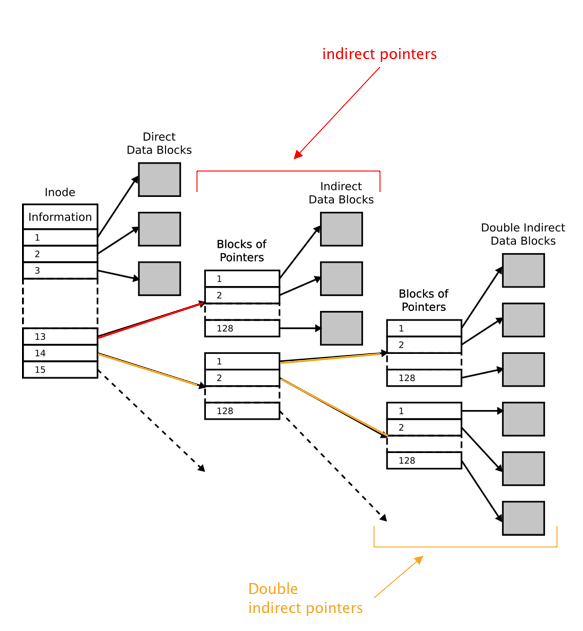
\includegraphics[width=\linewidth]{../images/midterm_2_solution_25.png}
    \end{center}
\end{itemize}

\section{Triple Indirect Pointers}

\begin{itemize}
    \item is allocated when double indirect pointer is not large enough
    \item has $1024^3$ pointers
    \item each of $1024^3$ pointers point to 4KB data block
    \item File can grow to be $(12 + 1024 + 1024^2 + 1024^3) \times 4\text{K} = 4299165744\text{KB}$ or $\approx 4.00 \text{TB}$
\end{itemize}

\section{Old UNIX File system}
\begin{itemize}
    \item was simple, and looked like the following on disk

    \begin{center}
    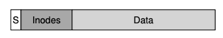
\includegraphics[width=0.6\linewidth]{../images/midterm_2_solution_26.png}
    \end{center}
    \item has terrible performance
    \item suffers from \textbf{external fragmentation}
    \item had small data block (512 bytes) and transfer of data took too long
\end{itemize}

\section{Fast File System}

\begin{itemize}
    \item modern file system has same APIS (\texttt{read()}, \texttt{write()}, \texttt{open()}, \texttt{close()})
    \item divides into a number of \textbf{cylinder groups}

    \begin{center}
    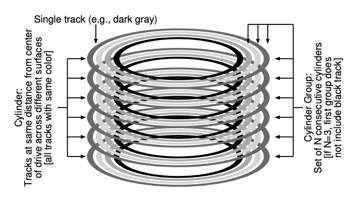
\includegraphics[width=0.8\linewidth]{../images/midterm_2_solution_28.png}
    \end{center}
    \item each \textbf{block group} or \textbf{cylinder group} is consecutive
    portion of disk's address

    \begin{center}
    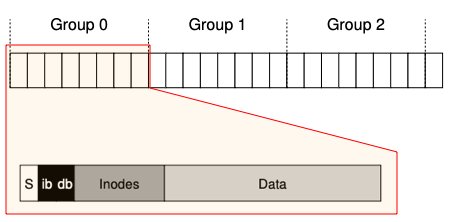
\includegraphics[width=0.8\linewidth]{../images/midterm_2_solution_29.png}
    \end{center}
\end{itemize}

\section{Bitmap}

\begin{itemize}
    \item Are excellent way to \underline{manage free space}
    \item tracks whether inodes/data block of the group are allocated
\end{itemize}

\section{FFS Policies: Allocating Files and Directories}

\begin{itemize}
    \item Basic Idea: keep related stuff together, and keep related stuff
    far apart
    \item Directories Step

    \begin{enumerate}[1)]
        \item Find the \textbf{cylinder group} with a low number of allocated directories
        and a high number of free inodes

        \begin{itemize}
            \item low number of allocated directories $\to$ to balance directories
            across groups
            \item high number of free nodes $\to$ to subsequently be able to allocate a bunch offiles
        \end{itemize}
        \item Put directory data and inode to the \textbf{cylinder group}
    \end{enumerate}

    \item Files Step

    \begin{enumerate}[1)]
        \item Allocate the data blocks of a file in the same \textbf{cylinder group} as its inode
        \item Place all files in the same directory in the cylinder group of the directory they are in

        \bigskip

        \underline{\textbf{Example}}

        \bigskip

        On putting \texttt{/a/c}, \texttt{/a/d}, \texttt{/b/f}, FFS would place

        \begin{itemize}
            \item \texttt{/a/c}, \texttt{/a/d} as close as possible in the same \textbf{cylinder group},
            \item \texttt{/b/f} located far away (in some other \textbf{cylinder group})
        \end{itemize}
    \end{enumerate}
\end{itemize}

\section{Inode}

\begin{center}
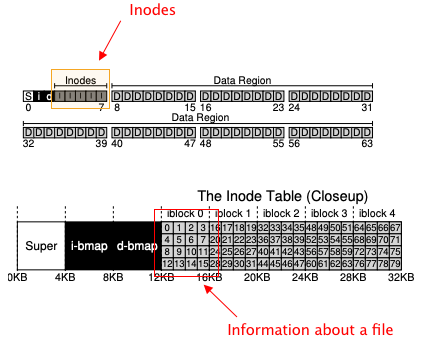
\includegraphics[width=\linewidth]{../images/midterm_2_solution_30.png}
\end{center}

\begin{itemize}
    \item Is a short form for \textbf{index node}
    \item Contains disk block location of the object's data $^{[1]}$
    \item Contains all the information you need about a file (i.e. metadata)

    \begin{itemize}
        \item File Type
        \begin{itemize}
            \item e.g. regular file, directory, etc
        \end{itemize}
        \item Size
        \item Number of blocks allocated to it
        \item Protection information
        \begin{itemize}
            \item such as who owns the file, as well as who can access it
        \end{itemize}
        \item Time information
        \begin{itemize}
            \item e.g. When file was created, modified, or last accessed
        \end{itemize}
        \item Location of data blocks reside on disk
    \end{itemize}
\end{itemize}

\section{Crash Consistency}

\begin{itemize}
    \item Goal: How to update persistent data structures despite the presence of
    a \textbf{power loss} or \textbf{system crash}?
\end{itemize}

\section{Crash Scenarios}

\begin{center}
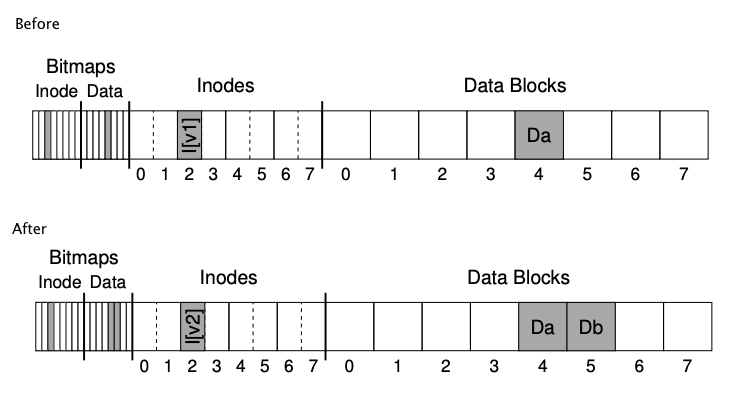
\includegraphics[width=\linewidth]{../images/midterm_2_solution_31.png}
\end{center}


\begin{enumerate}[1)]
    \item Just the data block (Db) is written to disk

    \bigskip

    \begin{itemize}
        \item No inode that points to it
        \item No bitmap that says the block is allocated
        \item It is as if the write never occured
        \item There is no problem here. All is well. (In file system's point of view)
    \end{itemize}

    \bigskip

    \item Just the updated inode (I[v2]) is written to disk

    \bigskip

    \begin{itemize}
        \item Inode points to the disk where \texttt{Db} is about to be written
        \item No bitmap that says the block is allocated
        \item No \texttt{Db} is written
        \item Garbage data will be read
        \item Also creates \textbf{File-system Inconsistency}

        \begin{itemize}
            \item Caused by on-disk bitmap telling us Db 5 is not allocated,
            but inode saying it does
        \end{itemize}
    \end{itemize}

    \bigskip

    \item Just the updated bitmap (B[v2]) is written to disk

    \bigskip

    \begin{itemize}
        \item Bitmap indicates tht block 5 is allocated
        \item No inode exists at block 5
        \item Creates \textbf{file-system inconsistency}
        \item Creates \textbf{space-leak} if left as is

        \begin{itemize}
            \item block 5 can never be used by the file system
        \end{itemize}
    \end{itemize}

    \bigskip

    \item Inode (I[v2]) and bitmap (B[v2]) are written to disk, and not data

    \bigskip

    \begin{itemize}
        \item File system metadata is completely consistent (in perspective of file system)
        \item Garbage data will be read
    \end{itemize}

    \bigskip

    \item Inode (I[v2]) and data block (Db) are written, but not the bit map

    \bigskip

    \begin{itemize}
        \item Creates \textbf{file-system inconsistency}
        \item Needs to be resolved before using file system again
    \end{itemize}

    \bigskip

    \item Bitmap (B[v2]) and data block (Db) are written, but not the inode (I[v2])

    \bigskip

    \begin{itemize}
        \item Creates \textbf{file-system inconsistency} between inode and data bitmap
        \item Creates \textbf{space-leak} if left as is
        \begin{itemize}
            \item Inode block is lost for future use
        \end{itemize}
        \item Creates \textbf{data-leak} if left as is

        \begin{itemize}
            \item Data block is lost for future use
        \end{itemize}
    \end{itemize}
\end{enumerate}

\section{External Fragmentation}

\begin{itemize}
    \item Is various free holes that are generated in either your
    memory or disk space. $^{[8]}$
    \item Are available for allocation, but may be too small to be of
    any use $^{[8]}$
\end{itemize}

\section{Internal Fragmentation}

\begin{itemize}
    \item Is wasted space within each allocated block $^{[8]}$
    \item Occurs when more computer memory is allocated than is needed
\end{itemize}

\*section{Extent Based File System}

\begin{center}
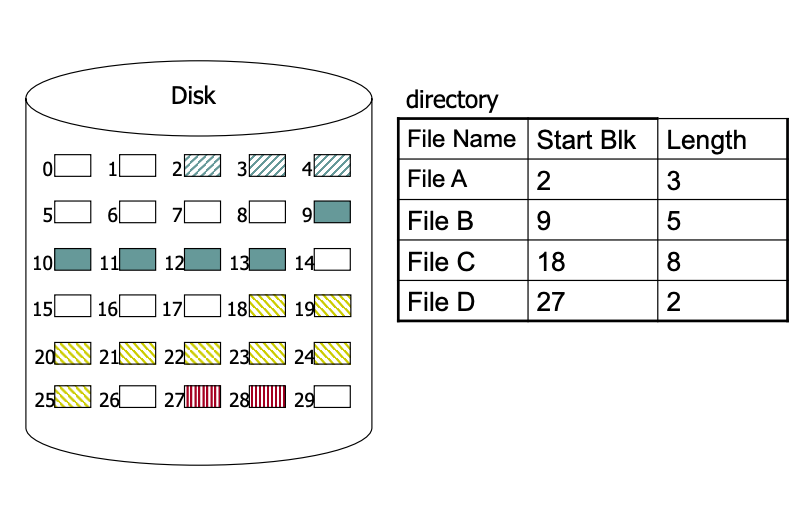
\includegraphics[width=\linewidth]{../images/midterm_2_solution_32.png}
\end{center}

\begin{itemize}
    \item Is simply a disk pointer plus a length (in blocks)
    \begin{itemize}
        \item Together, is called \textbf{extent}
    \end{itemize}
    \item Often allows more than one extent
    \begin{itemize}
        \item resolve problem of finding continuous free blocks
    \end{itemize}
    \item Is less flexible but more compact
    \item Works well when there is enough free space on the disk and
    files can be laid out contiguously
\end{itemize}

\bigskip

\underline{\textbf{Example}}

\bigskip

Linux's ext4 file system

\*section{Fields}

\begin{itemize}
    \item Is the members in a structure

    \bigskip

    \begin{center}
    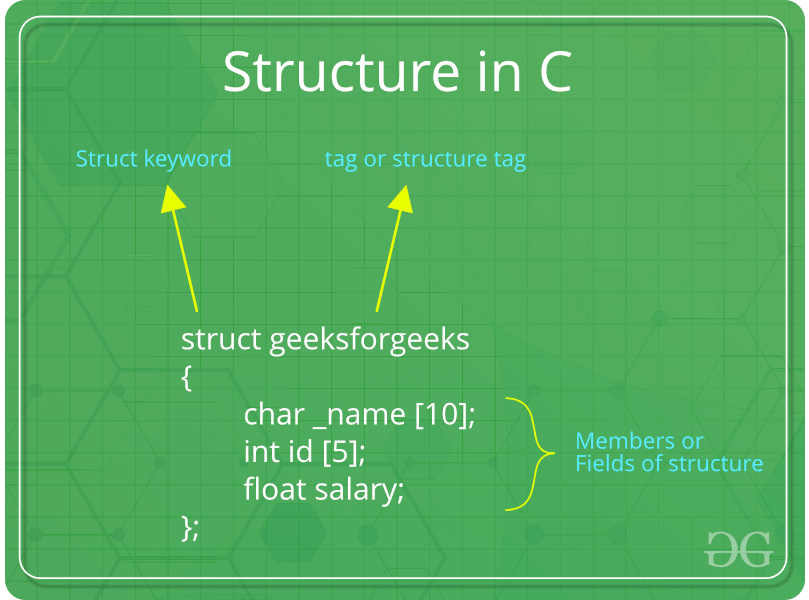
\includegraphics[width=0.6\linewidth]{../images/midterm_2_solution_33.png}
    \end{center}
\end{itemize}

\*section{Process List}

\begin{itemize}
    \item Is a data structure in kernel or OS
    \item Contains information about all the processes running in the system
\end{itemize}

\*section{Process Control Block}

\begin{itemize}
    \item Is a data structure in kernel or OS
    \item Contains all information about a process
    \item Is where the OS keeps all of a process' hardware execution state
    \item Generally includes

    \begin{enumerate}[1.]
        \item Process state (ready, running, blocked)
        \item Process number
        \item Program counter: address of the next instruction
        \item CPU Registers: is saved at an interrupt
        \item CPU scheduling information: process priority
        \item Memory management info: page tables
        \item I/O status information: list of open files
    \end{enumerate}
\end{itemize}

\end{document}
